\documentclass[border=10pt]{standalone}

\usepackage{tikz}
\usepackage{tikzsymbols}
\usetikzlibrary{calc,patterns,shapes.geometric}

\def\centerarc[#1](#2)(#3:#4:#5){\draw[#1] ($(#2)+({#5*cos(#3)},{#5*sin(#3)})$) arc (#3:#4:#5);}

\begin{document}
	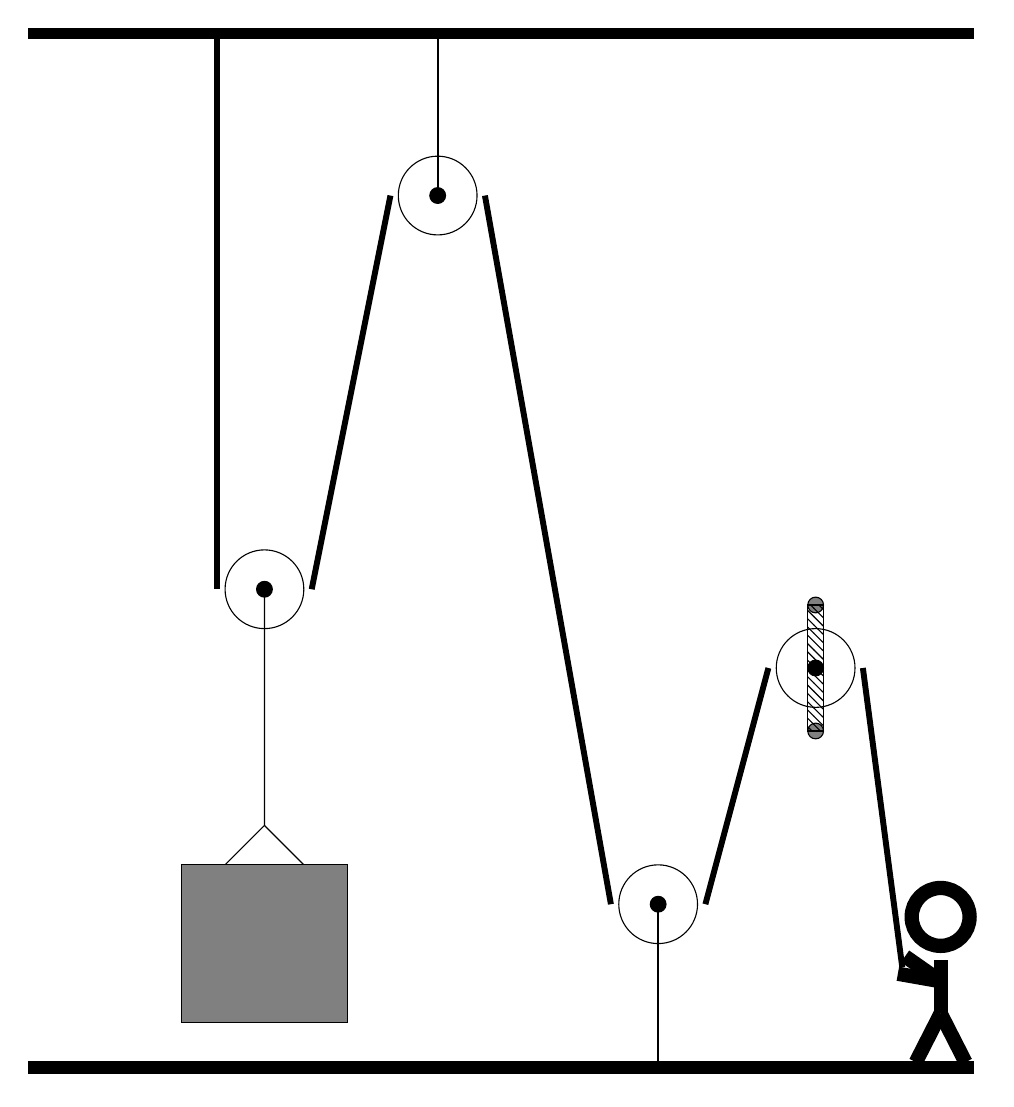
\begin{tikzpicture}
		%%%%% START %%%%%
		\draw[fill=black] (-2, 10) rectangle (10, 10.125);
		
		\draw (1, 3.0) circle (0.5);
		\draw[fill=black] (1, 3.0) circle (0.1);
		
		\draw (3.2, 8.0) circle (0.5);
		\draw[fill=black] (3.2, 8.0) circle (0.1);
		\draw[thick] (3.2, 8.0) -- (3.2, 10);
		
		\draw (6, -1) circle (0.5);
		\draw[fill=black] (6, -1) circle (0.1);
		\draw[thick] (6, -1) -- (6, -3);
		
		\draw[fill=white](8, 2.0) circle (0.5);
		\draw[fill=black] (8, 2.0) circle (0.1);
		\draw[fill=black!50] (8, 2.8) circle (0.1);
		\draw[fill=black!50] (8, 1.2) circle (0.1);
		\draw[pattern=north west lines, pattern color=black] (7.9, 2.8) rectangle (8.1, 1.2);
		
		\draw (1, 3.0) -- (1, 0) -- (0.5, -0.5);
		\draw (1, 0) -- (1.5, -0.5);
		\draw[fill=black!50] (-0.05, -0.5) rectangle (2.05, -2.5);
		
		\draw[line width=0.75mm] (0.4, 10) -- (0.4, 3.0);
		\centerarc[line width=0.75mm](1, 3.0)(180:360:0.6);
		\draw[line width=0.75mm](1.6, 3.0) -- (2.6, 8.0);
		\centerarc[line width=0.75mm](3.2, 8.0)(0:180:0.6);
		\draw[line width=0.75mm](3.8, 8.0) -- (5.4, -1);
		\centerarc[line width=0.75mm](6, -1)(180:360:0.6);
		\draw[line width=0.75mm](6.6, -1) -- (7.4, 2.0);
		\centerarc[line width=0.75mm](8, 2.0)(0:180:0.6);
		\draw[line width=0.75mm](8.6, 2.0) -- (9.1, -1.8);
		
		\node at (9.5, -1.9) {\Strichmaxerl[10][-35][170]};
		
		\draw[fill=black] (-2, -3) rectangle (10, -3.15);
		%%%%% END %%%%%
	\end{tikzpicture}
\end{document}